\usetikzlibrary{decorations.pathreplacing, positioning, calc}

% Definizioni dei colori campionati dall'immagine
\definecolor{labelred}{HTML}{D15545}
\definecolor{bracepurple}{HTML}{9B4582}

\chapter{Diagramma della Macchina a Stati}
\section{A cosa servono?}
I diagrammi di macchina a stati sono strumenti fondamentali utilizzati per modellare il comportamento dinamico di classificatori, come classi, casi d'uso, sottosistemi e interi sistemi.

Sono particolarmente utili per descrivere oggetti "reattivi" o complessi che possiedono un ciclo di vita definito da una precisa successione di stati, transizioni ed eventi

\section{Sintassi base}
\begin{center}
    \begin{tikzpicture}[
    font=\sffamily,
    node distance=1.5cm,
    state/.style={rectangle, draw, rounded corners=8pt, minimum width=1.5cm, minimum height=0.8cm},
    arrow/.style={-{Stealth}, thin}
]

    % Nodi
    \node[circle, fill=black, inner sep=2.5pt] (start) {};
    \node[state, right=of start] (A) {A};
    \node[state, right=2cm of A] (B) {B};
    \node[circle, draw, inner sep=1.5pt, right=of B] (end_outer) {};
    \node[circle, fill=black, inner sep=1.5pt] (end_inner) at (end_outer) {};

    % Transizioni
    \draw[arrow] (start) -- (A);
    \draw[arrow] (A) -- node[above, font=\small] (event) {unEvento} (B);
    \draw[arrow] (B) -- (end_outer);

    % Etichette (con linee sottili verso gli elementi)
    \draw[labelred, thin] (start) -- ++(-90:0.5) node[below] {Stato iniziale};
    \draw[labelred, thin] (event) -- ++(90:0.5) node[above] {evento};
    \draw[labelred, thin] (A) -- ++(-90:0.8) node[below] {transizione}; % Riferito all'arco
    \draw[labelred, thin] (B) -- ++(-90:0.5) node[below] {stato};
    \draw[labelred, thin] (end_outer) -- ++(-90:0.5) node[below] {Stato finale};

\end{tikzpicture}
\end{center}

\begin{itemize}
    \item Ogni macchina a stati dovrebbe avere uno stato iniziale che indica il primo stato della sequenza
    \item A meno che esista un ciclo perpetuo di stati, dovrebbe avere uno stato finale che termina la sequenza di transizioni
\end{itemize}

\section{Stati}
\subsection{Definizione}
Uno stato rappresenta una condizione o una situazione nella vita di un oggetto, durante la quale quest'ultimo soddisfa una condizione, esegue un'attività o è in attesa di un evento.

Lo stato corrente di un oggetto dipende dai suoi comportamenti passati e definisce come risponderà agli eventi futuri

Lo stato di un oggetto in qualsiasi momento è determinato da:
\begin{itemize}
    \item I valori dei suoi attributi
    \item Le relazioni che ha con altri oggetti
    \item Le attività che sta eseguendo
\end{itemize}

\subsection{Sintassi}
\begin{minipage}{0.45\textwidth}
    \begin{figure}[H]
        \centering
        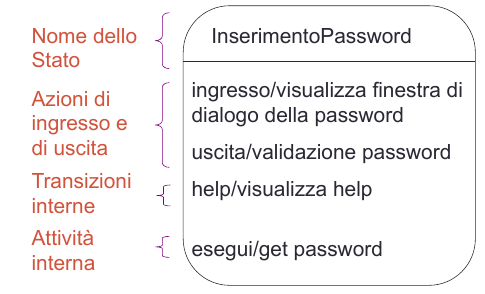
\includegraphics[scale=0.56]{Immagini/Schermata_20260709_165740.png}
    \end{figure}
\end{minipage}
\hfil
\begin{minipage}{0.45\textwidth}
    \begin{itemize}
        \item Le azioni sono istantanee e non interrompibili
        \item Le transizioni interne occorrono dentro lo stato. \\
        Non causano la transizione in un nuovo stato
        \item Le attività richiedono un intervallo di tempo finito e sono interrombpibili
    \end{itemize}
\end{minipage}

\section{Eventi}
\subsection{Definizione}
Un evento è la specifica di un occorrenza di interesse che ha una collocazione nel tempo e nello spazio

Gli eventi attivano le transizione e possono essere di 4 tipi
\subsection{Tipologie di eventi}
\subsubsection{Eventi di Chiamata}
\begin{minipage}{0.5\textwidth}
    \begin{figure}[H]
    \centering
    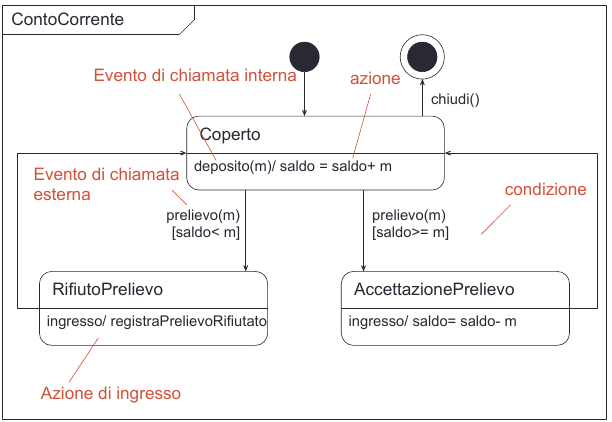
\includegraphics[scale=0.65]{Immagini/Schermata_20260709_171057.png}
\end{figure}
\end{minipage}
\hfil
\begin{minipage}{0.35\textwidth}
\begin{itemize}
    \item Rappresentano la chiamata a una specifica operazione.\\
    \item Affinchè siano validi, l'evento dovrebbe avere la stessa segnatura di un'operazione della classe di contesto in cui si trova la macchina a stati
\end{itemize}
\end{minipage}

\subsubsection{Eventi di Segnale}
\begin{minipage}{0.5\textwidth}
    \begin{figure}[H]
        \centering
        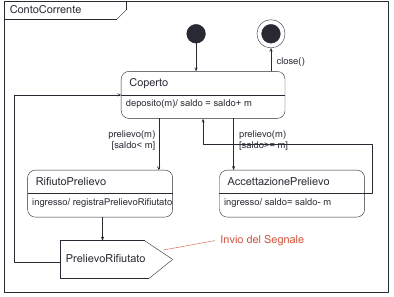
\includegraphics{Immagini/Schermata_20260709_171630.png}
    \end{figure}
    \begin{figure}[H]
        \centering
        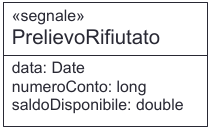
\includegraphics[scale=0.7]{Immagini/Schermata_20260709_171843.png}
    \end{figure}
\end{minipage}
\hfil
\begin{minipage}{0.35\textwidth}
    \begin{itemize}
        \item Un segnale è un pacchetto di informazioni inviato in modo asincrono tra oggetti \\
        \item I suoi attributi contengono le informazioni da trasportare e, graficamente, la sua ricezione è indicata da un pentagono concavo
    \end{itemize}
\end{minipage}

\subsubsection{Eventi di Variazione}
\begin{minipage}{0.5\textwidth}
    \begin{figure}[H]
        \centering
        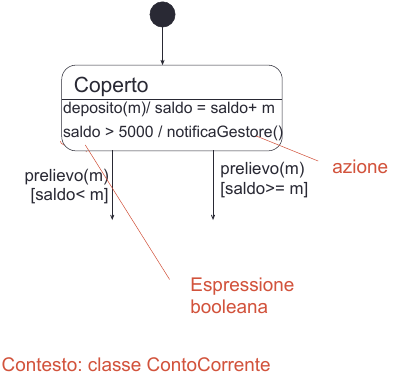
\includegraphics{Immagini/Schermata_20260709_172422.png}
    \end{figure}
\end{minipage}
\hfil
\begin{minipage}{0.35\textwidth}
    \begin{itemize}
        \item Sono rappresentati da un'espressione booleana continua.\\
        \item La transizione scatta nell'esatto momento in cui il valore dell'espressione passa da falso a vero \\
        \item Implementativamente, questo richiede un ciclo di test continuo per tutta la durata dello stato
    \end{itemize}
\end{minipage}

\subsubsection{Eventi Temporali}
\begin{minipage}{0.5\textwidth}
    \begin{figure}[H]
        \centering
        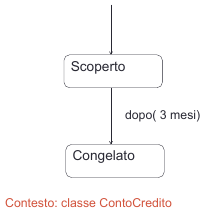
\includegraphics{Immagini/Schermata_20260712_102556.png}
    \end{figure}
\end{minipage}
\hfil
\begin{minipage}{0.35\textwidth}
    \begin{itemize}
        \item Gli eventi temporali occorrono quando un espressione di tempo diventa vera \\
        \item Le parole chiavi sono, dopo e quando
    \end{itemize}
\end{minipage}

\newpage
\section{Stati Composti}
\subsection{Definizione}
Uno stato composto è uno stato che contiene al suo interno una o sotto-macchine a stati (regioni).

Vengono utilizzati per organizzare e semplificare sistemi complessi, evitando la proliferazione di transizione ripetitive e introducendo concentti avanzati come l'ereditarietà delle transizioni, la scomposizione gerarchica e la concorrenza

\subsection{Stati Composti Semplici (Non-Ortogonali)}
\begin{minipage}{0.5\textwidth}
    \begin{figure}[H]
        \centering
        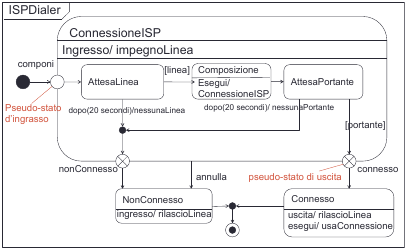
\includegraphics{Immagini/Schermata_20260712_103204.png}
    \end{figure}
\end{minipage}
\hfil
\begin{minipage}{0.35\textwidth}
    \begin{itemize}
        \item Contengono una solo regione di sotto-stati. \\

        \item Quando l'oggetto si trova nel super-stato, può essere attivo uno e un solo sotto-stato interno alla volta
    \end{itemize}
\end{minipage}

\subsection{Stati Composti Ortogonali}
    \begin{figure}[H]
        \centering
        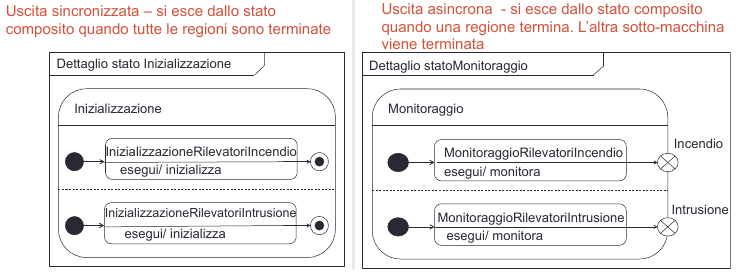
\includegraphics{Immagini/Schermata_20260712_103505.png}
    \end{figure}
    \begin{itemize}
        \item Contengono due o più regioni parallele (separate graficamente da una linea tratteggiata)\\

        \item Quando si entra in uno stato ortogonale, l'oggetto si trova contemporaneamente in un sotto-stato di ciascuna regione. \\
        \item Quando serve modellare attività concorrenti o indipendenti dello stesso oggetto
    \end{itemize}

\section{Sottomacchine}
\subsection{Cosa sono?}Come visto in precedenza, uno stato composito può contenere al suo interno una o più "sotto-macchine" annidate (suddivise in regioni).

Tuttavia, modellare sistemi complessi disegnando tutte le sottomacchine all'interno di un unico grande diagrammo lo renderebbe rapidamente enrome e illegibile

\subsection{Stati della Sotto Macchina}
\begin{minipage}{0.5\textwidth}
    \begin{figure}[H]
        \centering
        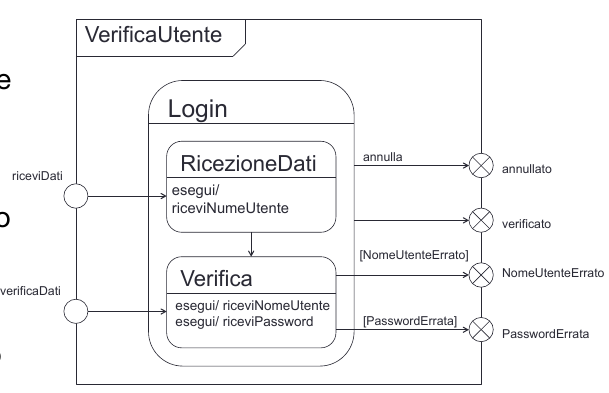
\includegraphics[scale=0.7]{Immagini/Schermata_20260712_104134.png}
    \end{figure}
\end{minipage}
\hfil
\begin{minipage}{0.35\textwidth}
    \begin{itemize}
        \item Se vogliamo fare riferimento a questa macchina a stati in altre macchine a stati, senza ingombrare i diagrammi, dobbiamo usare gli stati della sotto-macchine \\

        \item Gli stati della sotto-macchina fanno riferimento a un'altra macchina a stati \\
        \item Gli stati della sotto-macchina sono semanticamente equivalenti agli stati composti
    \end{itemize}
\end{minipage}

\subsection{Sintassi degli stati della Sotto-Macchine}
\begin{minipage}{0.5\textwidth}
    \begin{figure}[H]
        \centering
        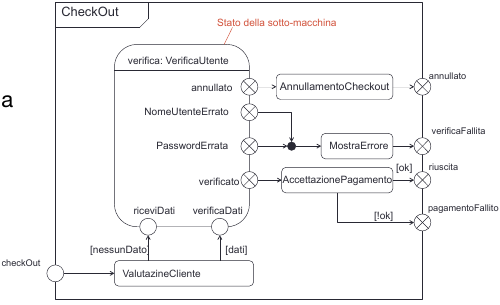
\includegraphics[scale=0.85]{Immagini/Schermata_20260712_104408.png}
    \end{figure}
\end{minipage}
\hfil
\begin{minipage}{0.35\textwidth}
    \begin{itemize}
        \item Uno stato della sotto-macchina è equivalente a includere una copia della sotto-macchina al posto dello stato della sotto-macchina
    \end{itemize}
\end{minipage}

\subsection{Comunicazione tra sotto-macchine}
\begin{figure}[H]
    \centering
    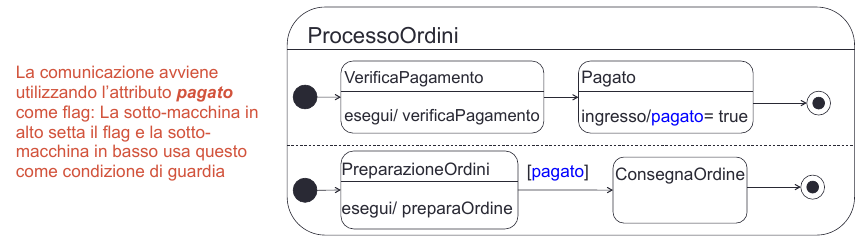
\includegraphics[scale=0.8]{Immagini/Schermata_20260712_104621.png}
\end{figure}
\begin{itemize}
    \item Capita spesso di avere l'esigenza di far comunicare due sotto-macchine
    \item Biforcazioni e ricongiunzioni possono essere utilizzate per creare sotto-macchine concorrenti e per risincronizzare
    \item La communicazione asincrona è ottenuta da una sotto-macchina configurando un flag per un altra sotto-macchine
\end{itemize}

\subsection{Comunicazione tramite stato di sync}
\begin{figure}[H]
    \centering
    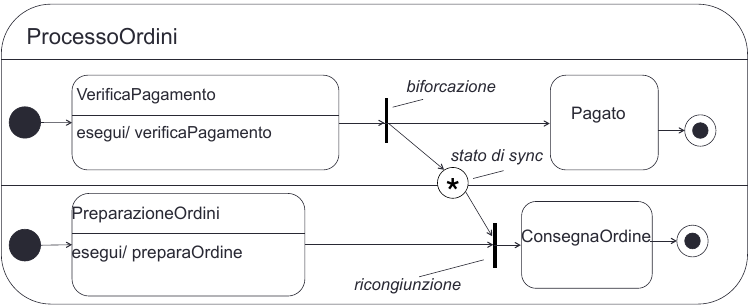
\includegraphics[scale=0.8]{Immagini/Schermata_20260712_104914.png}
\end{figure}
\begin{itemize}
    \item Lo stato di sync è uno stato speciale il cui compito è quello di tenere traccia di ogni singola attivazione della sua unica transizione di input
    \item Lo stato di sync è come una coda: si aggiunge un elemento alla coda ogni volta che viene attiviata la transizione di input
    \begin{itemize}
        \item numero limitato di elementi specificando all'interno dello stato di sync un numero intero positivo
        \item Asterisco per un numero illimitato di elementi
    \end{itemize}
\end{itemize}

\newpage
\subsection{Stati con memoria semplice}
\begin{figure}[H]
    \centering
    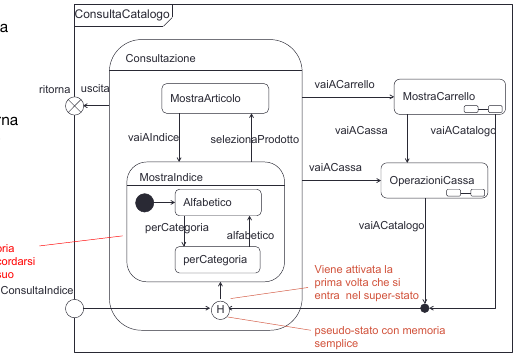
\includegraphics{Immagini/Schermata_20260712_105246.png}
\end{figure}
\begin{itemize}
    \item Lo pseudo-stato con memoria semplice ricorda in quale sottostato si era quando si è lasciato il super-stato
    \item In seguito quando si ritorna da uno stato esterno allo stato con memoria, l'indicatore ridirezione la transizione sull'ultimo sottostato memorizzato
\end{itemize}
\subsection{Sottostato con memoria multilivello}
\begin{figure}[H]
    \centering
    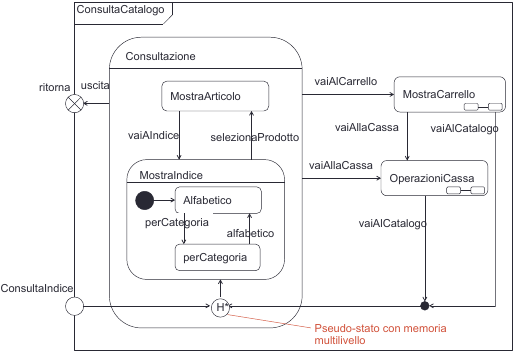
\includegraphics{Immagini/Schermata_20260712_105557.png}
\end{figure}
Uno stato con memoria multilivello può non solo ricordarsi l'ultimo sottostato attivo allo stesso livello dello pseudo-stato ma anche l'eventuale ultimo sottostato attivo di questo stato attivo e così via

\section{Esempio: Elabora vendita}
\begin{figure}[H]
    \centering
    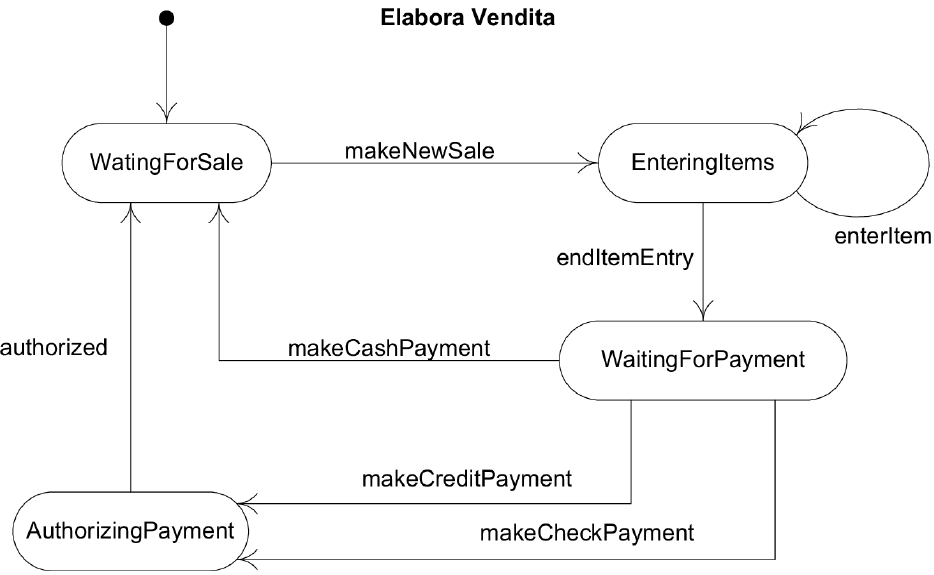
\includegraphics[scale=0.7]{Immagini/Schermata_20260712_105752.png}
\end{figure}